\section{Discrete-Time Systems\buch{Chapter 3}}
\subsection{Linearity and time invariance\buchSeite{100-102}}
\begin{tabular}{ll}
\textbf{Linearity:} & $x(n) = ax_1(n) + bx_2(n) \quad \underrightarrow{H} \quad y(n) = ay_1(n) + by_2(n)$\\
\textbf{Time invariance:} & If $y(n) = x(n)$ then $y(n+\delta) = x(n+\delta)$\\
testing: & $x_D(n)=x(n-D)$ and $y_D(n)=y(n-D)$\\
\end{tabular}

\subsection{Impulse response\buchSeite{103-105}}
\begin{tabular}{ll}
	\textbf{LTI form:}		& $y(n) = \sum\limits_m x(m)h(n-m)$ \\
	\textbf{direct form:}	& $y(n) = \sum\limits_m h(m)x(n-m)$
\end{tabular}


\subsection{Finite and Infinite Impulse Response filters\buchSeite{105,106}}
\begin{tabularx}{0.75\textwidth}{|l|X|X|}
	\hline
	$M$	& filter order				& 
	\\ \hline
	$h$	& filter impulse response	& $\{ h_0, h_1, h_2, \ldots , h_M, 0, 0, \ldots\}$
	\\ \hline
	$L_h$	& length of $h$			& $L_h = M + 1$
	\\ \hline
	FIR		& FIR filtering equation	& $y(n) = \sum\limits_{m=0}^{M} h(m)x(n-m)$
	\\ \hline
	IIR		& IIR filtering equation	& $y(n) = \sum\limits_{m=0}^{\infty} h(m)x(n-m)$
	\\ \hline
\end{tabularx}

\begin{multicols}{2}
\subsection{Causality\buchSeite{112}}
\begin{tabular}{lp{4.5cm}}
	\textbf{causal} & right sided signals, they are non-zero for $n>=0$ \\
	\textbf{anticausal} & left sided signals, they are non-zero for $n<=-1$ \\
	\textbf{mixed signals} & double-sided signals \\
\end{tabular}
\vfill

\columnbreak

\subsubsection{Anticausal to Causal\buchSeite{113}}
Delay the system by $D$ to move the negative time from $n=-D$ to $0$
\begin{align*}
h_D(n) =& h(n-D)\\
y(n) =& \sum\limits_{m}h(m)x(n-m) \\
y_D(n) = & \sum\limits_{m}h_D(m)x(n-m) = \sum\limits_{m}h(m-D)x(n-m) \\ 
\xrightarrow{m := k+D}& \sum\limits_{k}h(k)x(n-k-D) = y(n-D)
\end{align*}
\end{multicols}
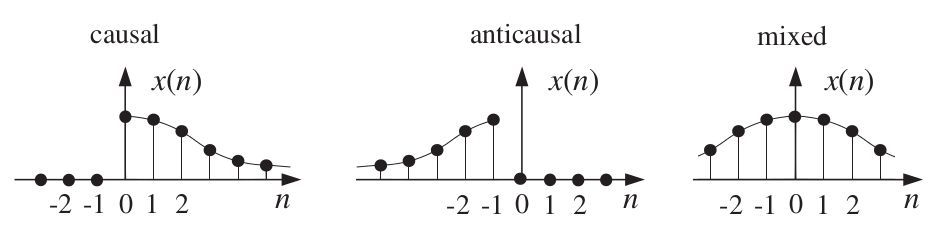
\includegraphics[width=15cm]{./picture/causality}

\subsection{Stability\buchSeite{115}}
\textbf{Stability Condition} $\sum\limits_{n=-\infty}^{\infty}\left| h(n)
\right| < \infty$\\
An LTI system is stable, if a bounded input can only generate bounded outputs.
Always prefer stability over causality!
